% Created by tikzDevice version 0.12.3.1 on 2021-12-06 10:55:33
% !TEX encoding = UTF-8 Unicode
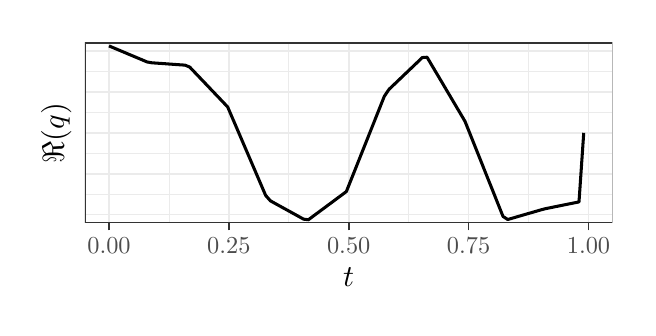
\begin{tikzpicture}[x=1pt,y=1pt]
\definecolor{fillColor}{RGB}{255,255,255}
\path[use as bounding box,fill=fillColor,fill opacity=0.00] (0,0) rectangle (216.81,101.18);
\begin{scope}
\path[clip] (  0.00,  0.00) rectangle (216.81,101.18);
\definecolor{drawColor}{RGB}{255,255,255}
\definecolor{fillColor}{RGB}{255,255,255}

\path[draw=drawColor,line width= 0.6pt,line join=round,line cap=round,fill=fillColor] (  0.00,  0.00) rectangle (216.81,101.18);
\end{scope}
\begin{scope}
\path[clip] ( 20.71, 30.69) rectangle (211.31, 95.68);
\definecolor{fillColor}{RGB}{255,255,255}

\path[fill=fillColor] ( 20.71, 30.69) rectangle (211.31, 95.68);
\definecolor{drawColor}{gray}{0.92}

\path[draw=drawColor,line width= 0.3pt,line join=round] ( 20.71, 41.03) --
	(211.31, 41.03);

\path[draw=drawColor,line width= 0.3pt,line join=round] ( 20.71, 55.80) --
	(211.31, 55.80);

\path[draw=drawColor,line width= 0.3pt,line join=round] ( 20.71, 70.57) --
	(211.31, 70.57);

\path[draw=drawColor,line width= 0.3pt,line join=round] ( 20.71, 85.34) --
	(211.31, 85.34);

\path[draw=drawColor,line width= 0.3pt,line join=round] ( 51.04, 30.69) --
	( 51.04, 95.68);

\path[draw=drawColor,line width= 0.3pt,line join=round] ( 94.35, 30.69) --
	( 94.35, 95.68);

\path[draw=drawColor,line width= 0.3pt,line join=round] (137.67, 30.69) --
	(137.67, 95.68);

\path[draw=drawColor,line width= 0.3pt,line join=round] (180.99, 30.69) --
	(180.99, 95.68);

\path[draw=drawColor,line width= 0.6pt,line join=round] ( 20.71, 33.64) --
	(211.31, 33.64);

\path[draw=drawColor,line width= 0.6pt,line join=round] ( 20.71, 48.41) --
	(211.31, 48.41);

\path[draw=drawColor,line width= 0.6pt,line join=round] ( 20.71, 63.18) --
	(211.31, 63.18);

\path[draw=drawColor,line width= 0.6pt,line join=round] ( 20.71, 77.95) --
	(211.31, 77.95);

\path[draw=drawColor,line width= 0.6pt,line join=round] ( 20.71, 92.72) --
	(211.31, 92.72);

\path[draw=drawColor,line width= 0.6pt,line join=round] ( 29.38, 30.69) --
	( 29.38, 95.68);

\path[draw=drawColor,line width= 0.6pt,line join=round] ( 72.69, 30.69) --
	( 72.69, 95.68);

\path[draw=drawColor,line width= 0.6pt,line join=round] (116.01, 30.69) --
	(116.01, 95.68);

\path[draw=drawColor,line width= 0.6pt,line join=round] (159.33, 30.69) --
	(159.33, 95.68);

\path[draw=drawColor,line width= 0.6pt,line join=round] (202.65, 30.69) --
	(202.65, 95.68);
\definecolor{drawColor}{RGB}{0,0,0}

\path[draw=drawColor,line width= 1.1pt,line join=round] ( 29.38, 94.59) --
	( 31.09, 93.87) --
	( 32.81, 93.15) --
	( 34.52, 92.43) --
	( 36.24, 91.70) --
	( 37.96, 90.98) --
	( 39.67, 90.26) --
	( 41.39, 89.54) --
	( 43.10, 88.81) --
	( 44.82, 88.49) --
	( 46.53, 88.37) --
	( 48.25, 88.25) --
	( 49.96, 88.13) --
	( 51.68, 88.00) --
	( 53.40, 87.88) --
	( 55.11, 87.76) --
	( 56.83, 87.64) --
	( 58.54, 86.96) --
	( 60.26, 85.15) --
	( 61.97, 83.35) --
	( 63.69, 81.55) --
	( 65.40, 79.75) --
	( 67.12, 77.94) --
	( 68.84, 76.14) --
	( 70.55, 74.34) --
	( 72.27, 72.53) --
	( 73.98, 68.54) --
	( 75.70, 64.54) --
	( 77.41, 60.55) --
	( 79.13, 56.55) --
	( 80.84, 52.56) --
	( 82.56, 48.56) --
	( 84.27, 44.57) --
	( 85.99, 40.57) --
	( 87.71, 38.61) --
	( 89.42, 37.66) --
	( 91.14, 36.71) --
	( 92.85, 35.77) --
	( 94.57, 34.82) --
	( 96.28, 33.88) --
	( 98.00, 32.93) --
	( 99.71, 31.98) --
	(101.43, 31.77) --
	(103.15, 33.05) --
	(104.86, 34.32) --
	(106.58, 35.59) --
	(108.29, 36.86) --
	(110.01, 38.13) --
	(111.72, 39.41) --
	(113.44, 40.68) --
	(115.15, 41.95) --
	(116.87, 46.25) --
	(118.59, 50.56) --
	(120.30, 54.86) --
	(122.02, 59.17) --
	(123.73, 63.47) --
	(125.45, 67.78) --
	(127.16, 72.08) --
	(128.88, 76.39) --
	(130.59, 78.92) --
	(132.31, 80.55) --
	(134.03, 82.19) --
	(135.74, 83.83) --
	(137.46, 85.47) --
	(139.17, 87.10) --
	(140.89, 88.74) --
	(142.60, 90.38) --
	(144.32, 90.50) --
	(146.03, 87.60) --
	(147.75, 84.70) --
	(149.47, 81.81) --
	(151.18, 78.91) --
	(152.90, 76.01) --
	(154.61, 73.11) --
	(156.33, 70.21) --
	(158.04, 67.31) --
	(159.76, 63.02) --
	(161.47, 58.72) --
	(163.19, 54.43) --
	(164.90, 50.14) --
	(166.62, 45.84) --
	(168.34, 41.55) --
	(170.05, 37.26) --
	(171.77, 32.96) --
	(173.48, 31.86) --
	(175.20, 32.36) --
	(176.91, 32.86) --
	(178.63, 33.36) --
	(180.34, 33.86) --
	(182.06, 34.35) --
	(183.78, 34.85) --
	(185.49, 35.35) --
	(187.21, 35.80) --
	(188.92, 36.14) --
	(190.64, 36.49) --
	(192.35, 36.83) --
	(194.07, 37.18) --
	(195.78, 37.52) --
	(197.50, 37.87) --
	(199.22, 38.21) --
	(200.93, 63.18);
\definecolor{drawColor}{gray}{0.20}

\path[draw=drawColor,line width= 0.6pt,line join=round,line cap=round] ( 20.71, 30.69) rectangle (211.31, 95.68);
\end{scope}
\begin{scope}
\path[clip] (  0.00,  0.00) rectangle (216.81,101.18);
\definecolor{drawColor}{gray}{0.20}

\path[draw=drawColor,line width= 0.6pt,line join=round] ( 29.38, 27.94) --
	( 29.38, 30.69);

\path[draw=drawColor,line width= 0.6pt,line join=round] ( 72.69, 27.94) --
	( 72.69, 30.69);

\path[draw=drawColor,line width= 0.6pt,line join=round] (116.01, 27.94) --
	(116.01, 30.69);

\path[draw=drawColor,line width= 0.6pt,line join=round] (159.33, 27.94) --
	(159.33, 30.69);

\path[draw=drawColor,line width= 0.6pt,line join=round] (202.65, 27.94) --
	(202.65, 30.69);
\end{scope}
\begin{scope}
\path[clip] (  0.00,  0.00) rectangle (216.81,101.18);
\definecolor{drawColor}{gray}{0.30}

\node[text=drawColor,anchor=base,inner sep=0pt, outer sep=0pt, scale=  0.88] at ( 29.38, 19.68) {0.00};

\node[text=drawColor,anchor=base,inner sep=0pt, outer sep=0pt, scale=  0.88] at ( 72.69, 19.68) {0.25};

\node[text=drawColor,anchor=base,inner sep=0pt, outer sep=0pt, scale=  0.88] at (116.01, 19.68) {0.50};

\node[text=drawColor,anchor=base,inner sep=0pt, outer sep=0pt, scale=  0.88] at (159.33, 19.68) {0.75};

\node[text=drawColor,anchor=base,inner sep=0pt, outer sep=0pt, scale=  0.88] at (202.65, 19.68) {1.00};
\end{scope}
\begin{scope}
\path[clip] (  0.00,  0.00) rectangle (216.81,101.18);
\definecolor{drawColor}{RGB}{0,0,0}

\node[text=drawColor,anchor=base,inner sep=0pt, outer sep=0pt, scale=  1.10] at (116.01,  7.64) {$t$};
\end{scope}
\begin{scope}
\path[clip] (  0.00,  0.00) rectangle (216.81,101.18);
\definecolor{drawColor}{RGB}{0,0,0}

\node[text=drawColor,rotate= 90.00,anchor=base,inner sep=0pt, outer sep=0pt, scale=  1.10] at ( 13.08, 63.18) {$\Re(q)$};
\end{scope}
\end{tikzpicture}
